\section{Gothenburg --- Gothenburg Congestion Tax}

\subsection{History}

The genesis of Gothenburg's pricing system lies in the above-mentioned infrastructure agreement between Stockholm and the national government. Previously, most infrastructure projects in Sweden were funded nationally, but the agreement demonstrated a local/national co-financing model that proved attractive in an era of restricted budgets \citep{Borjesson2015,Hysing2015b}. In 2008 the government directed the national infrastructure administrations to prioritize such co-financing when selecting projects for the 2010-2021 transport investment plan. When a draft of the plan came out in spring 2009, leaders from the Gothenburg region lamented that many of their high-priority projects had been left out, and embarked on negotiations with national officials about co-financing these projects. The negotiations proceed quickly, and in October 2009 the Gothenburg City Council ratified the ``West Swedish Agreement,'' whereby 17 billion SEK in local funds---including 14 billion from road pricing---would be matched one-for-one by national funds. The Agreement included a 20 billion SEK rail tunnel (the ``Western Link''), a road tunnel, bus lanes and a multi-modal bridge. 

Unlike the protracted process behind the Stockholm Congestion tax, the selection of projects and the design of the road pricing scheme were both rushed, so that the projects could be included in the national investment plan that Parliament passed in April 2010. This provoked controversy, and in the September 2010 elections, voters gave several seats on the Gothenburg City Council to a new party, Vägvalet (``Road Selection''), whose sole issue was opposition to road pricing. In 2012, a public petition drive led the council to  place a on-binding referendum on the coming charges on the 2014 election ballot. Nevertheless, the Council pressed ahead, and the Gothenburg Congestion Tax (GCT) launched on January 1st, 2013 with a design copied from the SCT.

In September 2014, the referendum result showed 57\% of votes cast were against continuing the charge, but since the referendum was only consultative, the Council decided to keep the Tax in order to fulfill Gothenburg's end of the West Swedish Agreement. This motive has been well illustrated by the decision to increase tolls in January 2015 after early revenues fell short of projections.

\subsection{Design}

Gothenburg's scheme closely resembles Stockholm's: cameras identify drivers crossing tolling sites in either direction, and tolls vary by time-of-day. Figure XXX shows the tolling schedule before and after the 2015 increase. There is a daily maximum charge of 60 SEK, and the same vehicles are exempt as in Stockholm. The ``single charge'' or  ``multi-passage'' rule declares that, no matter how many tolling sites a vehicle crosses within 60 minutes, it is charged only once, with the toll being the highest among the possible charges. Figure \ref{fig:Gothenburg-map} shows the tolling sites form a cordon around downtown Gothenburg, but there are also sites at the \"Alvsborg Bridge (toll site \#11) and along a highway north of the city where congestion would otherwise be severe. 

\begin{figure}[ht]
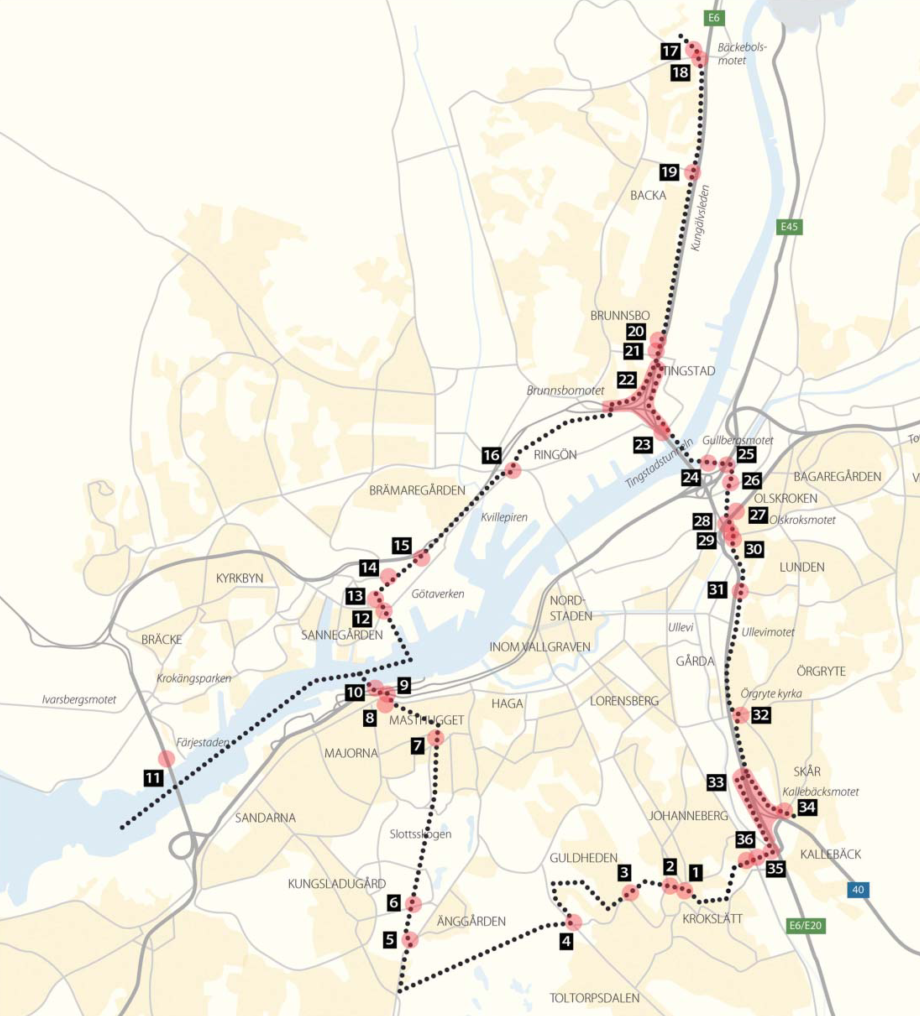
\includegraphics[width=0.7\textwidth]{../img/gburg-map.png}

\caption{Gothenburg Congestion Tax zone \citep{transportstyrelsen2015}\label{fig:Gothenburg-map}}
\end{figure}

\subsection{Results}

The effects in Gothenburg were similar to but milder than those observed in Stockholm. Traffic over the cordon during the charged hours fell 12\%, rather than the 15\% forecast by models \citep{Borjesson2015}. The discrepancy was largest during the peaks: whereas models had predicted peak travel would fall 18\%, it fell only 13\%---approximately the same reduction observed for off-peak traffic. Travel surveys show that commuters switched to public transport, while discretionary travelers traveled less frequently or switched destinations. Accounting for external factors, the charge is estimated to have raised public transport ridership by about 4.5-6.5\%. As for congestion, Figure \ref{fig:Gothenburg-travel-times} shows travel times in Gothenburg for different classes of road from before and after the charge. Likewise, in Stockholm commuters switched to public transport, public transport ridership rose by about 5\%, discretionary travelers canceled trips, peak and off-peak traffic fell by similar amounts and travel time reductions were strongest on inner arterial roads.

\begin{figure}[ht]
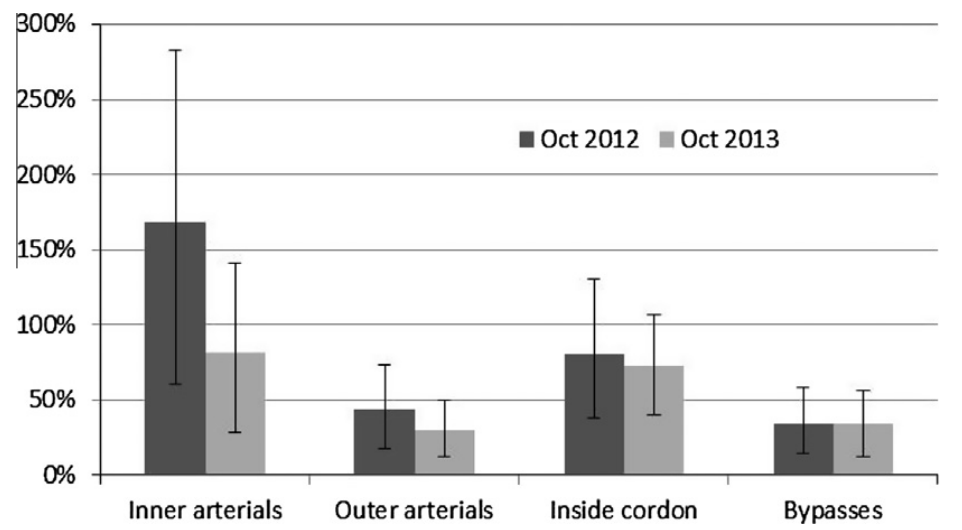
\includegraphics[width=0.55\columnwidth]{../img/gburg-travel-times.png}

\caption{Gothenburg 7-8AM. Increase in travel times on selected categories of road relative to free-flow speeds, before (Oct 2012) and after (Oct 2013) the Congestion Tax. \citep{Borjesson2015} \label{fig:Gothenburg-travel-times}}

\end{figure}

\subsection{Finances}

The GCT cost only 41 million EUR to implement if we count only those costs specific to Gothenburg \citep[p. 40]{Borjesson2018}. However, in 2012, Sweden spent 35 million EUR to replace the IT system for the Stockholm Congestion Tax with a national system that Gothenburg and two bridges elsewhere in Sweden could also use; arguably some part of this expense could be attributed to Gothenburg, too. 

In the first year, 2013, the GCT generated only 72 million EUR in charges and about 8 million EUR in penalties, instead of the 93 million EUR forecast in 2009 \citep[pp. 142-143]{Borjesson2015}. \citet{Borjesson2015} blame economic factors (fuel prices, recession) and the fact that 45\% of trips took advantage of the ``multi-passage'' rule rather than the 30\% analysts predicted. After the toll increase in 2015, revenues jumped from 80 million EUR in 2014 to 99.5 million EUR in 2015, while operating costs have stayed around 13 million EUR per year \citep[table 3]{Borjesson2018}.

% Operating costs have been low: 

% In any case, the expense compares very favorably to implementation costs in Singapore (XXX), London (XXX) and Stockholm (XXX), which illustrates the value of experience.









% When the GCT was introduced, Sweden scrapped the 

% In 2013 the Gothenburg Congestion Tax raised 846 million kr, of which 76 million kr came from tolls and 83.8 million kr from penalties \citep{TransportstyrelsenGburg2013}. This was short of the 930 million kr (\$103 million) forecast, largely because 45\% of traffic turned out to be exempt rather than the 30\% forecast \citep{Borjesson2015}.

% Since Gothenburg's 


\section{Discussion}\label{sec:discussion}

This chapter has reviewed the history of zone pricing from its conception as an idea in the 1950's and 1960's to its proliferation in the new millenium as a result of number-plate recognition technology. Surveying the zone pricing experience, two themes emerge that are worth highlighting.

First, note that all the systems surveyed produced similar traffic reductions, between 10 and 20 percent of all entries. This is surprising given that the amount of money charged varies considerably. In Stockholm, the maximum charge is only about \$3. In London it was about \$18 before the recent devaluation of the pound. Moreoever, the models in Stockholm and Gothenburg were mistaken in that they predicted different traffic reductions in the peak and off-peak, due to the time-varying toll. Instead what was observed is that a similar share of traffic stopped driving at both times of day. As a rule-of-thumb, it might be worthwhile to assume that, in any pre-charging population of drivers, about 10-15\% of drivers are simply unwilling to pay anything to drive, almost regardless of the size of the toll.

Second, while most of the theory of congestion pricing focuses on prices, in practice exemptions are critical. Some of these exemptions---such as those for the handicapped or medical vehicles---are easy to justify by appeals to welfare or social justice. But many exemptions---such as those for taxis or even, in the case of Milan, refrigerated delivery trucks---lack much of a rationale outside politics.
